\documentclass[a3paper,14pt]{article}
\usepackage[utf8]{inputenc}
\usepackage{extsizes}
\usepackage[T2A]{fontenc}
\usepackage[english,russian]{babel} 
\usepackage[left=15mm, top=25mm, right=15mm, bottom=25mm, nohead, nofoot]{geometry}
\usepackage{graphicx}
\usepackage{nicefrac}
\usepackage{tikz}
\usepackage{amsmath,amsfonts,amssymb} % математический пакет
\usepackage{fancybox,fancyhdr} % хедер и футер
\pagestyle{fancy}
\fancyhf{}
\fancyhead[L]{Дифференциальные уравнения}
\fancyhead[R]{Овчинников Павел, вариант 6}
\fancyfoot[C]{\thepage}
\setcounter{page}{1}
\headsep=10mm 
\usepackage{hyperref}
\usepackage{cancel}

\newlength{\tempheight}
\newcommand{\Let}[0]{
\mathbin{\text{\settoheight{\tempheight}{\mathstrut}\raisebox{0.4\pgflinewidth}{
\tikz[baseline=0.5ex,line cap=round,line join=round] \draw (0,0) --++ (0.3em,0) --++ (0,2.3ex) --++ (-0.3em,0);
}}}}
\newcommand*\squared[1]{\tikz[baseline=(char.base)]{
            \node[shape=rectangle,draw,inner sep=4pt] (char) {$#1$};}}
\newcommand{\at}{\biggr\rvert}

\begin{document}
\begin{titlepage}
    \begin{center}
        Министерство образования и науки Российской Федерации \\
        Федеральное государственное автономное образовательное учреждение \\ высшего образования \\[6pt]
        САНКТ-ПЕТЕРБУРГСКИЙ НАЦИОНАЛЬНЫЙ \\ ИССЛЕДОВАТЕЛЬСКИЙ УНИВЕРСИТЕТ ИТМО \\[16pt]
        Факультет систем управления и робототехники \\[25em]
        \textbf{РАСЧЁТНО-ГРАФИЧЕСКАЯ РАБОТА №1\\ПО РЕШЕНИЮ ДИФФЕРЕНЦИАЛЬНЫХ УРАВНЕНИЙ}
    \end{center}\,\\[12em]
    \begin{flushright}
        Студент: Овчинников П. А.\\
        Группа: R3241 \\
        Вариант №6 \\
        Преподаватель: Шиманская Г.С.
    \end{flushright}\,\\[13em]
    \begin{center}
        {\small Санкт-Петербург \\ 2023}
    \end{center}    
\end{titlepage}
\subsection*{\centering Задание №1}
\textbf{а)} $(y^2+3)\,dx-\dfrac{e^x}{x}y \,dy = 0$ \\
Перед нами простое дифференциальное уравнение, в котором достаточно будет перенести соответствующие слагаемые с каждой из переменных по разные стороны и затем проинтегрировать обе части:
$$(y^2+3)\,dx=\frac{e^x}{x}y \,dy$$
$$\frac{x}{e^x}\,dx=\frac{y}{y^2+3}\,dy$$
$$\int\frac{x}{e^x}\,dx=\int\frac{y}{y^2+3}\,dy$$
$$\int\left.\frac{x}{e^x}\,dx\right.^\ast=\int\left.\frac{y}{y^2+3}\,dy\right.^{\ast\ast}$$
$$(\ast)\colon \int\frac{x}{e^x}\,dx=\begin{bmatrix}
        \int uv' = uv - \int u'v \\ u=x \Rightarrow u'=1 \\
        \;v'=\nicefrac{1}{e^x} \Rightarrow v=\nicefrac{-1}{e^x}\;
    \end{bmatrix}= \frac{-x}{e^x}-\int\frac{-1}{e^x}+C = \frac{-x}{e^x} - \frac{1}{e^x}+C=-\frac{x+1}{e^x}+C$$
$$(\ast\ast)\colon \int\frac{y}{y^2+3}\,dy = \begin{bmatrix}
        t = y^2 + 3 \\
        \;\nicefrac{dt}{dy} = 2y \Rightarrow \,dy = \nicefrac{dt}{2y}\;
    \end{bmatrix} = \int\frac{\cancel{y}\,dt}{2\cancel{y}\,t} = \frac{1}{2}\int\frac{dt}{t}=\frac{\ln\vert t\vert}{2}=\frac{\ln\left\vert y^2+3\right\vert}{2}$$
$$-\frac{x+1}{e^x}+C=\frac{\ln\left\vert y^2+3\right\vert}{2}$$
$$\ln\left\vert y^2+3\right\vert=-2\;\frac{x+1}{e^x}+C$$
$$y^2+3=e^{-2\;\nicefrac{x+1}{e^x}+C}$$
$$\squared{y=\pm\sqrt{e^{-2\;\nicefrac{x+1}{e^x}+C}-3}}$$\,\\[0.5em]
\textbf{b)} $y^2+x^2y'=x y y'$\\
Практически не очевидно, что здесь однородное уравнение. Для начала приведём его к виду однородного и затем решим по известному нам алгоритму:
$$y'y x-y'x^2=y^2$$
$$y x\frac{dy}{dx}-x^2\frac{dy}{dx}=y^2$$
$$y x\frac{dy}{dx}-x^2\frac{dy}{dx}=y^2\;\at\cdot dx$$
$$y x\,dy-x^2\,dy=y^2\,dx$$
$$(y x-x^2)\,dy=y^2\,dx$$
$$\text{Проверим на однородность: } \frac{dy}{dx} = \frac{y^2}{y x-x^2}\at_{:x^2}=\frac{\left(\nicefrac{y}{x}\right)^2}{\nicefrac{y}{x}-1}=\varphi\left(\frac{y}{x}\right)\ \checkmark\ \ \Rightarrow\ \  y=zx\quad dy=x\,dz+z\,dx$$
$$(zx^2-x^2)(x\,dz+z\,dx)=z^2x^2\,dx$$
$$zx^3\,dz-x^3\,dz+\cancel{z^2x^2\,dx}-zx^2\,dx=\cancel{z^2x^2\,dx}\at:x^2\quad(x \ne 0)$$
$$zx\,dz-x\,dz=z\,dx$$
$$\left(1-\frac{1}{z}\right)\,dz=\frac{dx}{x}$$
$$\int\left(1-\frac{1}{z}\right)\,dz=\int\frac{dx}{x}$$
$$\int\left(1\,dz-\frac{1}{z}\,dz\right)=\ln\vert x\vert + C$$
$$z-\ln\vert z\vert=\ln\vert x\vert + C \qquad \Rightarrow \left[z=yx\right] \Rightarrow \qquad \frac{y}{x}-\ln\left\vert \frac{y}{x}\right\vert=\ln\vert x\vert + C$$
$$\frac{y}{x}-\ln\vert y \vert+\cancel{\ln\vert x\vert}=\cancel{\ln\vert x\vert} + C$$
$$\squared{\dfrac{y}{x}-\ln\vert y \vert = C}$$ \pagebreak

\noindent \textbf{c)} $y'-y=e^x$ \\
Перед нами самое обычное линейное неоднородное уравнение. Решаем его, как и подобает, через замену:
$$\Let y = uv \ \Rightarrow\  uv'+u'v-uv=e^x$$
$$u(v'-v)+u'v=e^x$$
$$\Let v'-v = 0 \ \Rightarrow\  \frac{dv}{v}=dx \ \Rightarrow\ \int\frac{dv}{v}=\int dx \ \Rightarrow\ \ln\vert v\vert = x \ \Rightarrow\ v = e^x + C_1$$
$$u'e^x=e^x\at:e^x$$
$$u'=1 \ \Rightarrow\ u = x + C_2$$
$$y = uv = (e^x + C_1)(x + C_2) \ \Rightarrow\ \squared{y = x e^x + C}\quad(C = C_1C_2)$$
Итак, функция $y(x)$ найдена. Остаётся найти её частное решение в точке $(0, 1)$:
$$y(0) = 1 \ \Rightarrow\ 0\cdot e^0 + C = 1 \ \Rightarrow\ \squared{C = 1}$$\,\\[0.5em]
\textbf{d)} $xy'+2y+x^5y^3e^x = 0$\\
Похоже, перед нами уравнение Бернулли. Решаем его делением на $y^3$ со старшей степенью и последующей заменой на $z = y^{-2}$, чтобы получить линейное неоднородное уравнение, но для начала нужно избавиться от $x$ рядом с $y'$:
$$xy'+2y+x^5y^3e^x = 0 \at:x$$
$$y'+\frac{2y}{x}+x^4y^3e^x = 0 \at:y^3$$
$$\frac{y'}{y^3}+\frac{2}{x y^2}+x^4e^x = 0$$
$$\Let z = y^{-2} \ \Rightarrow\ z' = -2y^{-3}y'$$
$$\frac{z'\cancel{y^3}}{-2\cancel{y^3}}+\frac{2z}{x}+x^4e^x = 0$$
$$-\frac{z'}{2}+\frac{2z}{x}+x^4e^x = 0 \at \cdot(-2)$$
$$z'-\frac{4z}{x}-2x^4e^x = 0$$
$$\Let z = uv \ \Rightarrow\ z' = uv' + u'v$$
$$uv'+u'v-\frac{4uv}{x} - 2x^4e^x = 0$$
$$u\left(v'-\frac{4v}{x}\right)+u'v - 2x^4e^x = 0$$
$$\Let v'-\frac{4v}{x}=0 \ \Rightarrow\ \frac{dv}{4v}=\frac{dx}{x} \ \Rightarrow\ \int\frac{dv}{4v}=\int\frac{dx}{x} \ \Rightarrow\ \frac{\ln\vert v\vert}{4}=\ln\vert x\vert \ \Rightarrow\ v = e^{4\ln\vert x\vert} + C_1 = x^4 + C_1$$
$$u'x^4=2x^4e^x$$
$$\frac{du}{dx}=\frac{2\cancel{x^4}e^x}{\cancel{x^4}}$$
$$du=2e^x\,dx$$
$$\int du=\int2e^x\,dx$$
$$u=2e^x + C_2$$
$$z = uv = (x^4 + C_1)(2e^x + C_2) = 2e^xx^4 + C\quad(C = C_1C_2)$$
$$z = y^{-2} = 2e^xx^4 + C \ \Rightarrow\ \squared{y = \dfrac{\pm1}{\sqrt{2e^xx^4 + C}}}$$ \pagebreak

\subsection*{\centering Задание №2}
26. $y'=(y-1)x$ \\
Имеем функцию, которую приравняем к коэффициенту наклона $k$, чтобы получить ряд изоклинов:
$$y'=(y-1)x=k$$
$$y-1=\frac{k}{x}$$
$$y=\frac{k}{x} + 1$$
Выберем шаг $\Delta k = 0.5$ и точку старта $k_0 = 0$ и построим 10 изоклин дифференциального уравнения. Для простоты восприятия на графике, кроме изоклин, уже отмечены синим интегральная кривая дифференциального уравнения и поле направлений тонкими отрезками, которое строилось так же с шагами $(\Delta x, \Delta y) = (0.5, 0.5)$ под углом наклона $\arctan(k)$ к точкам, лежащим на изоклинах:
\begin{figure}[h]
    \centering 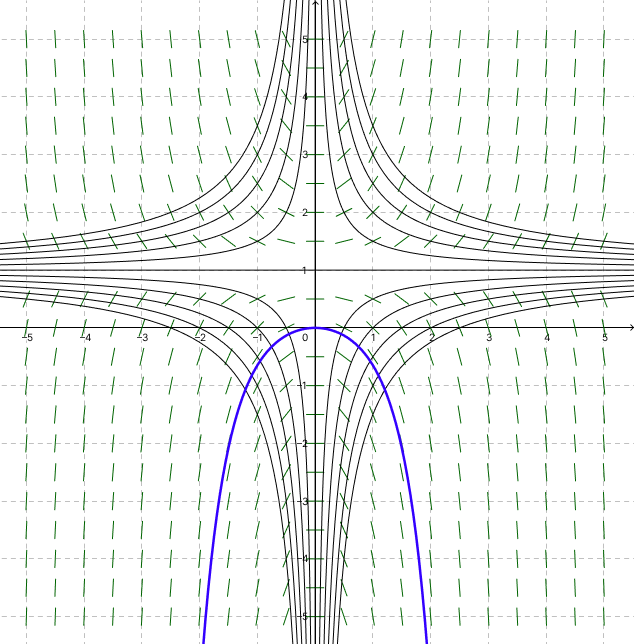
\includegraphics[width=0.5\textwidth]{isoclines.png}
    \caption{Рис. 1. Изоклины дифференциального уравнения $y'=(y-1)x$}
\end{figure}

\noindent Отмечу также, что ветви параболы могут идти и вверх --- здесь всё зависит от произвольной постоянной интегрирования $C$, которая может быть как отрицательной, так и положительной в решении этого уравнения $y = Ce^{\nicefrac{x^2}{2}}+1$. 

\end{document}